\section{Integration}

\begin{ILOssec}
    \item \ILOd
\end{ILOssec}

\subsection{Revision of basic integration}
\label{sec:basic_int}

\begin{learningoutcomes}
\item Calculate the definite and indefinite integral of basic mathematical functions
\end{learningoutcomes}

\textbf{Differentiation and Integration.} Integrating a function is the inverse of differentiation, and requires finding its ``anti-derivative''.

\[
x^3 \quad \xrightleftharpoons[\text{Integrate}]{\text{Differentiate}} \quad 3x^2.
\]

The integration is denoted as
\[
\int 3x^2\,{\rm d}x=x^3+C \, ,
\]
where $\int$ is the integral sign, $3x^2$ is the integrand, ${\rm d}x$ indicates integration with respect to $x$, and $x^3+C$ is the integral. The integral is not unique, the constant $C$ can take any value, since a constant differentiates to zero. This \textbf{constant of integration} must always be remembered when integrating.

\textbf{Differentiation vs. Integration.} Consider a function $y=f(x)$.
The process of differentiation gives information about its rate of change.
The process of integration gives information about the accumulation, $A(x)$, of the function, such that $A'(x) = f(x)$ (see figure \ref{fig:integration}).

Some standard integrals are given below
\[
\begin{array}{c|c}
\textbf{Function }y=f(x) & \textbf{Integral }\displaystyle\int f(x)\,{\rm d}x\\ \hline
x^n \; (n\neq-1)& \dfrac{1}{n+1}x^{n+1}+C\\[2mm]
\dfrac{1}{x} & \ln |x|+C\\[2mm]
e^x & e^x+C\\[2mm]
\sin x & -\cos x+C\\[2mm]
\cos x & \sin x+C\\[2mm]
\end{array}
\]

Using the chain rule for differentiation 
\[
\der{}{x} f(ax+b)=af'(ax+b) \, ,
\]
some of these can be generalised to the case of linear functions in the argument.
\[
\begin{array}{c|c}
\textbf{Function }y=f(x) & \textbf{Integral }\displaystyle\int f(x)\,{\rm d}x\\ \hline
e^{ax+b} & \dfrac{1}{a}e^{ax+b}+C\\[2mm]
\sin(ax+b) & -\dfrac{1}{a}\cos(ax+b)+C\\[2mm]
\cos(ax+b) & \dfrac{1}{a}\sin(ax+b)+C
\end{array}
\]

Some other standard integrals to be aware of are given below (and most are available in the mathematical formula tables). Note these can be derived using some of the techniques introduced later in this section.
\[
\begin{array}{c|c}
\textbf{Function }y=f(x) & \textbf{Integral }\displaystyle\int f(x)\,{\rm d}x\\ \hline
\tan x& \ln\left(\sec x\right) +C\\[2mm]
\dfrac{1}{a^2+x^2} & \dfrac{1}{a}\tan^{-1}\left(\dfrac{x}{a}\right) + C\\[2mm]
\dfrac{1}{\sqrt{a^2-x^2}}  & \sin^{-1}\left(\dfrac{x}{a}\right) + C\\[2mm]
\ln x \quad (x>0) & x \ln x - x + C
\end{array}
\]

\begin{figure}[h]
    \centering
    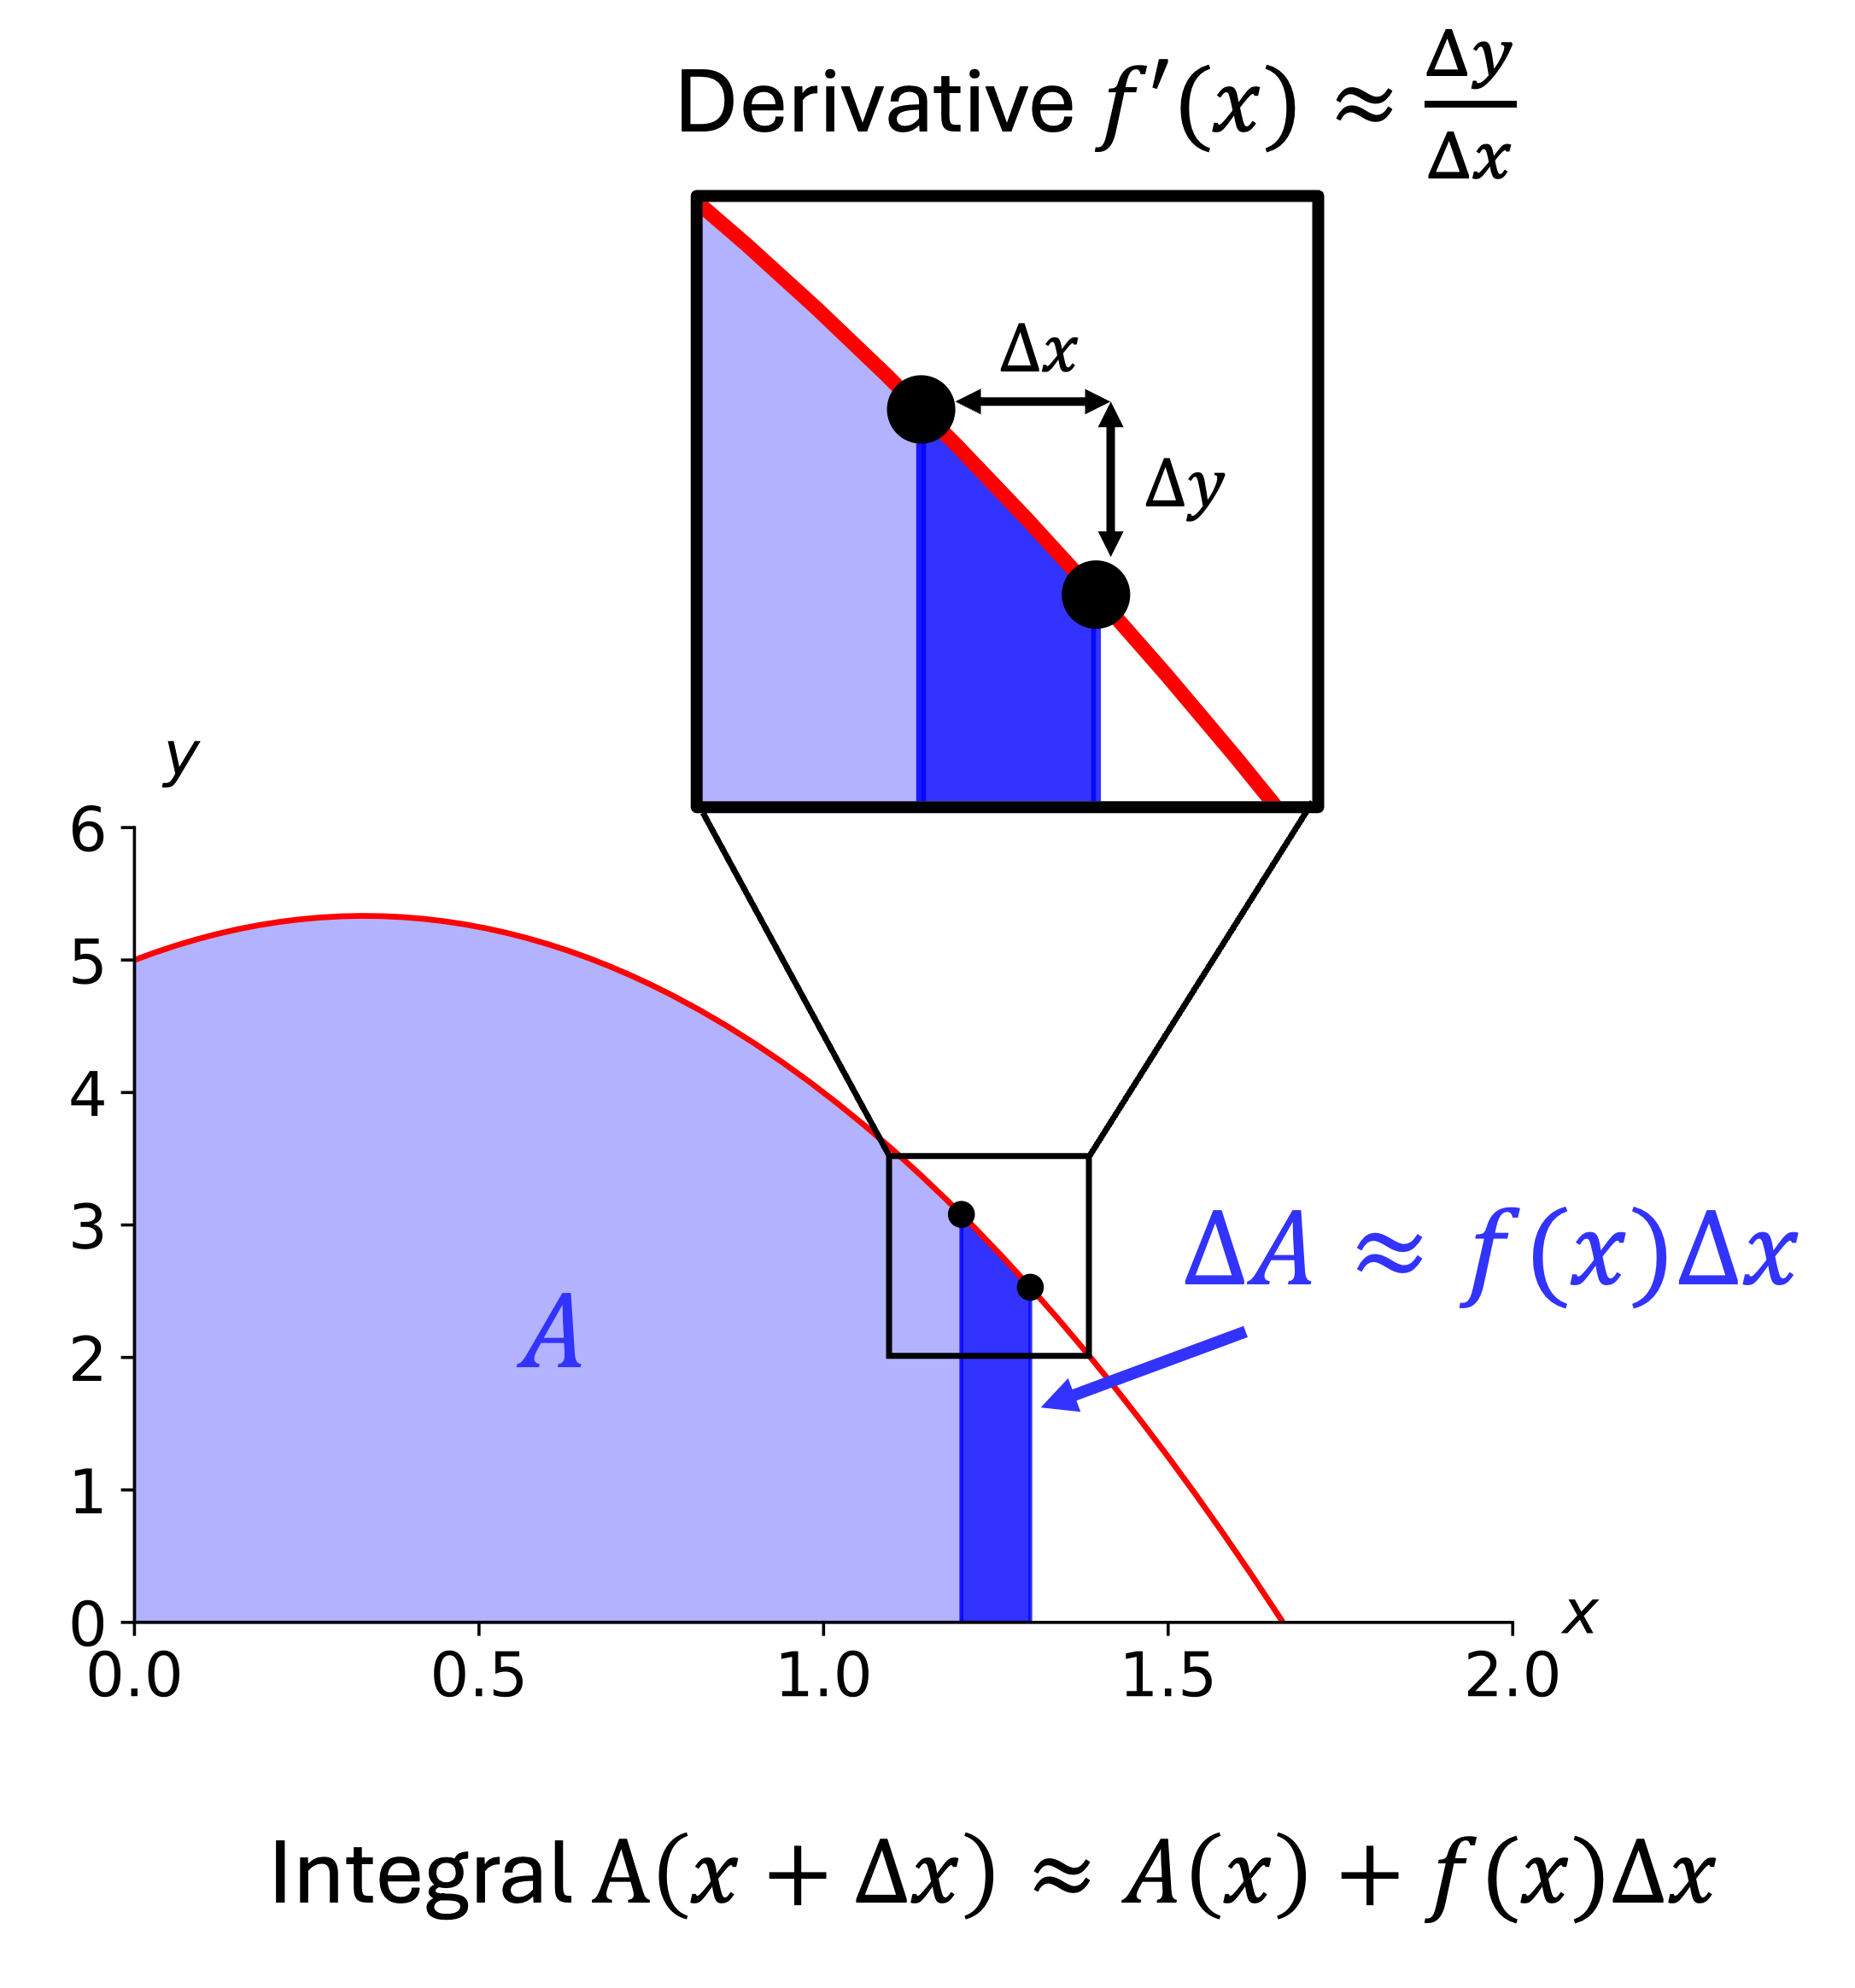
\includegraphics[width=0.5\linewidth]{Figures/Section3/311_integral.png}
    \caption{A sketch of the relationship between the derivative $f'(x)$ and the integral $f(x)$. If we zoom in, the curve is locally linear with gradient $\Delta y / \Delta x$ which is approximately equal to $f'(x)$. Integrating tells us how the area under the curve increases with $x$, so in moving from $x$ to $x+\Delta x$ we accrue an extra area of $\Delta A \approx f(x) \Delta x$. The integral is the sum of these thin strips in the limit $\Delta x \rightarrow 0$, which depends on where you begin the sum from, hence the need for a constant of integration, such that $\int f'(x) \, {\rm d} x = f(x)+C$. }
    \label{fig:integration}
\end{figure}

\textbf{Linearity of integration.} The integral of a sum of functions is equal to the sum of integrals
\[
\int[f(x)+g(x)]\,{\rm d}x=\int f(x)\,{\rm d}x+\int g(x)\,{\rm d}x.
\]

\begin{example}[Lecture]
Find the integral
\[
\int\left(4\cos x-3e^x\right)\,{\rm d}x.
\]
\end{example}

\begin{solution}
\[
\blank{4\sin x-3e^x+C}.
\]
\end{solution}

\textbf{The Definite Integral.} The definite integral uses the notation
\[
\int_a^b f(x)\,{\rm d}x.
\]
It measures how much the function has accumulated (or, equivalently, the area under the curve) between $x=a$ and $x=b$. The values $a$ and $b$ are referred to as the `limits of integration'. It is referred to as the ``integral from $a$ to $b$''.

To calculate the definite integral, first calculate the indefinite integral or  ``anti-derivative''.
\[
F(x)=\int f(x)\,{\rm d}x.
\]
Then, the definite integral is the difference between the indefinite integral at $a$ and $b$
\[
\int_a^b f(x)\,{\rm d}x=F(b)-F(a).
\]
Note, $F(x)$ contains a constant of integration, but this will always cancel out in the definite integral, so can be ignored.

It follows that the definite integral is additive, i.e. it can be `split up'. If $a<b<c$,
\[
\int_a^b f(x)\,{\rm d}x+\int_b^c f(x)\,{\rm d}x
=F(c)-F(b)+F(b)-F(a)
\]
\[
=F(c)-F(a)
\]
\[
=\int_a^c f(x)\,{\rm d}x.
\]

\begin{example}[Video]
A metal strip has width $w$ [cm] and is heated unevenly until it has a steady temperature field. The end of the strip is in contact with a conducting plate. The heat flux density at the interface is $kh$ where
\[
h=4+\left(\frac{x}{w}\right)^2-4\left(\frac{x}{w}\right)^3\;[\mathrm{W/cm}]
\]
where $0<x<w$ [cm].

Calculate the total heat flux
\[
H=k\int_0^w h\,{\rm d}x
\]
in terms of the conductivity $k$ and the width $w$.
% 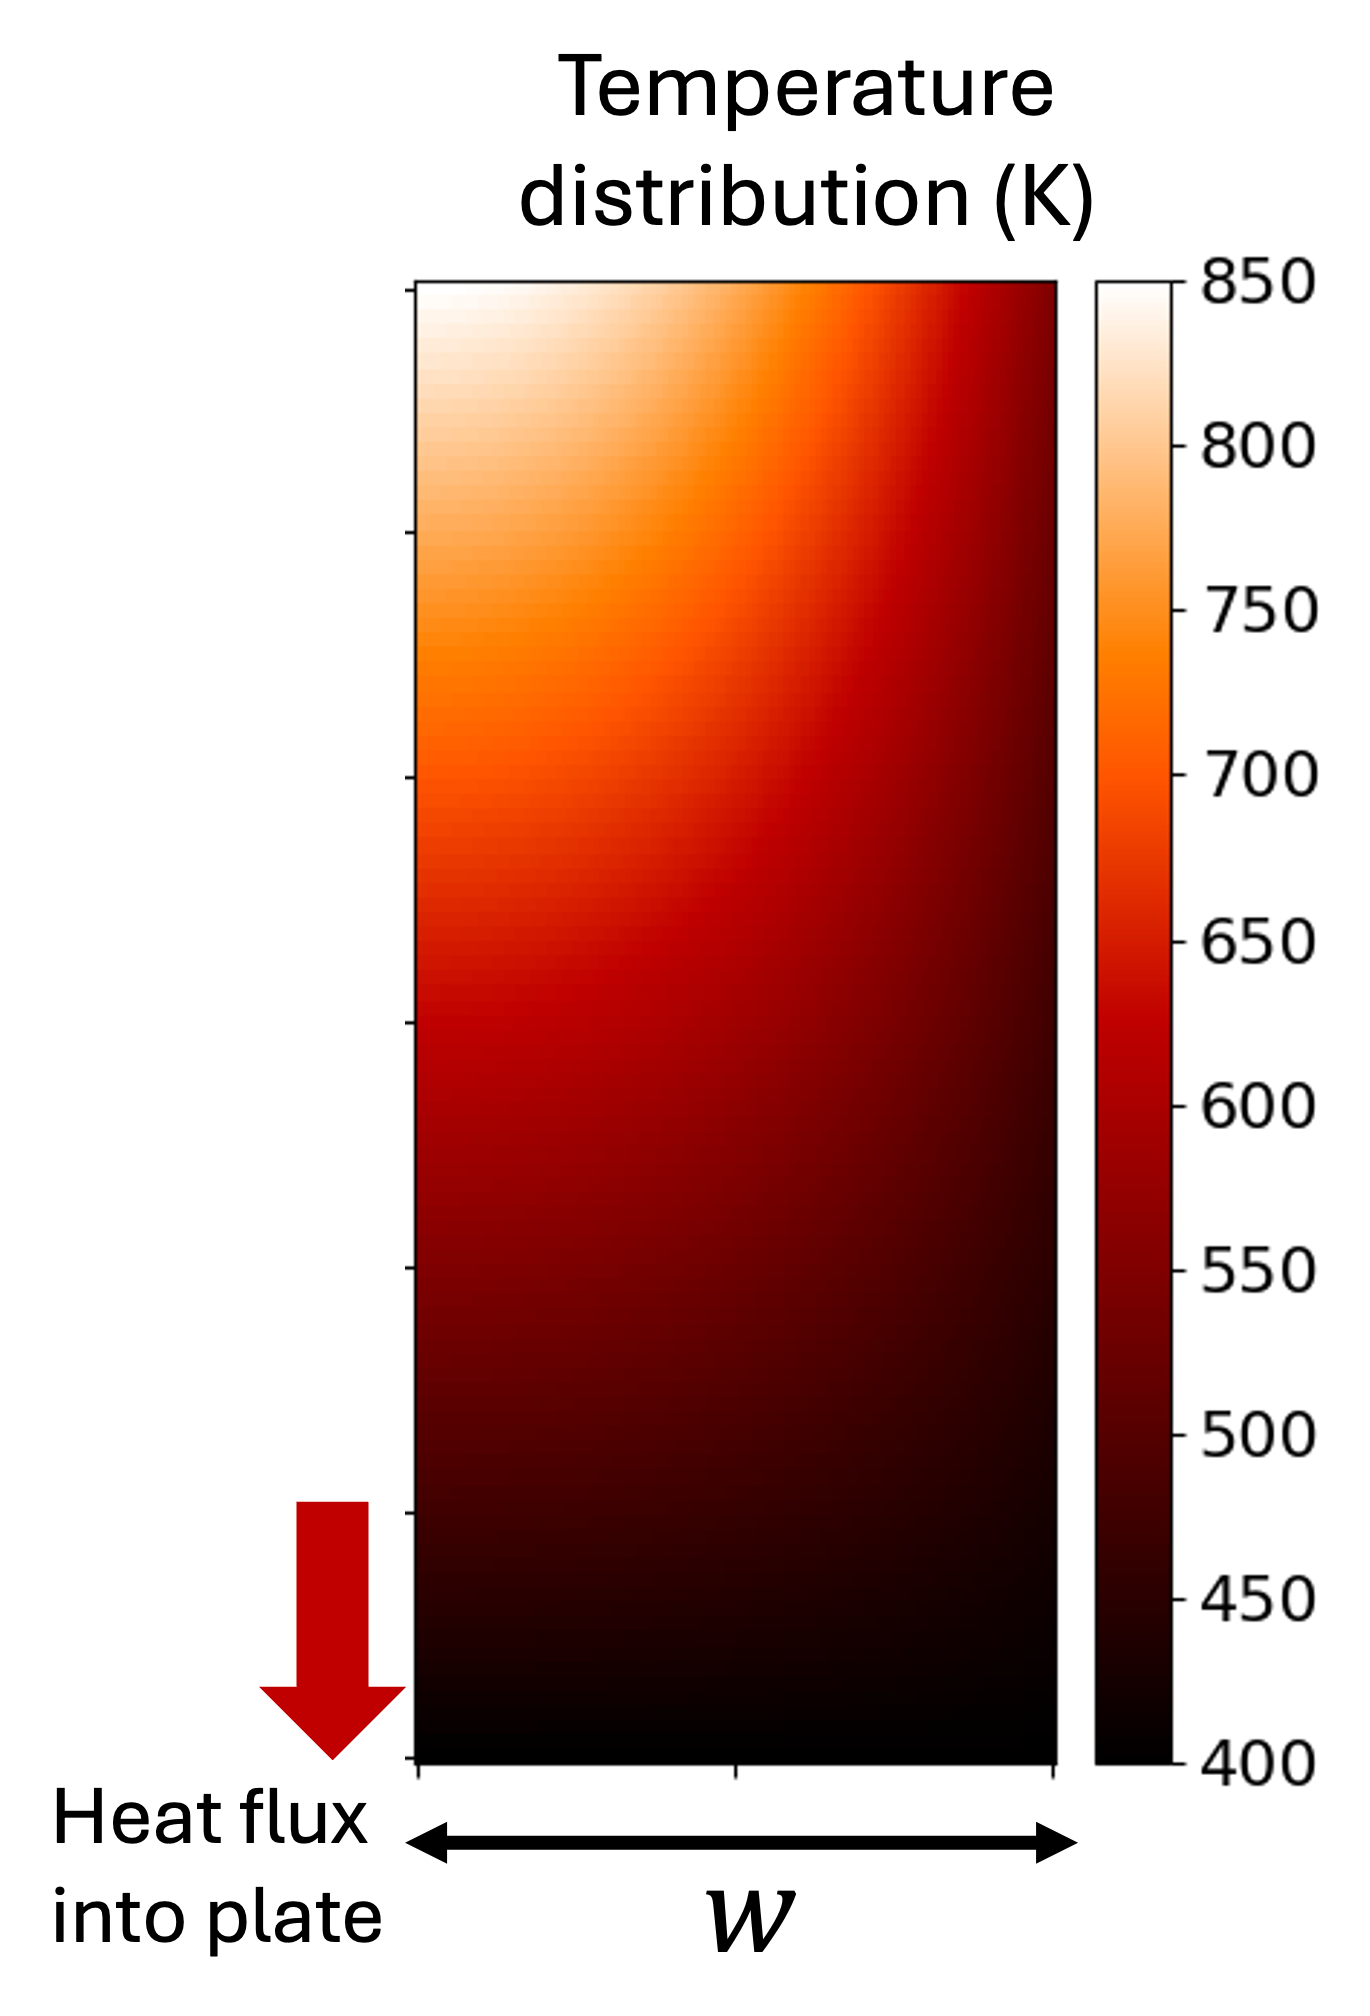
\includegraphics[width=0.25\textwidth,alt='Contour plot of the temperature in the strip']{Figures/Section3/Ex312.png}
\end{example}

\begin{solution}
Calculate the indefinite integral and substitute in the limits
\[
\int_0^w h\,{\rm d}x
=
\blank{\left[4x+\frac{x^3}{3w^2}-\frac{x^4}{w^3}\right]_0^w}
\]
\[
\blank{=4w+\frac{w}{3}-w}
\]
\[
\blank{=3w+\frac{w}{3}=\frac{10w}{3}}.
\]
Then
\[
H=k\int_0^w h\,{\rm d}x=\blank{\frac{10}{3}kw\;[\mathrm{W}]}.
\]
\end{solution}

\begin{recap}{\ref{sec:basic_int}}
\item Integration is the \textbf{reverse operation} to differentiation. \item Integration measures the \textbf{accumulation of a function}.
\item Indefinite integrals give rise to a \textbf{constant of integration}.
\item Definite integrals are calculated using the indefinite integral
\[
\int_a^b f(x)\,{\rm d}x=F(b)-F(a).
\]
\end{recap}

\subsection{Integration and areas defined by curves}
\label{sec:areas_int}

\begin{learningoutcomes}
\item Calculate the area under a curve and between curves using integration
\end{learningoutcomes}

The definite integral provides a way of finding the area under or above a curve or the area between curves.

\textbf{Area under a curve.} Consider the curve in figure \ref{fig:int_curve} defined by the function $y=f(x)$ for values of $x$ between the values $x=a$ and $x=b$.

\begin{figure}[h]
    \centering
    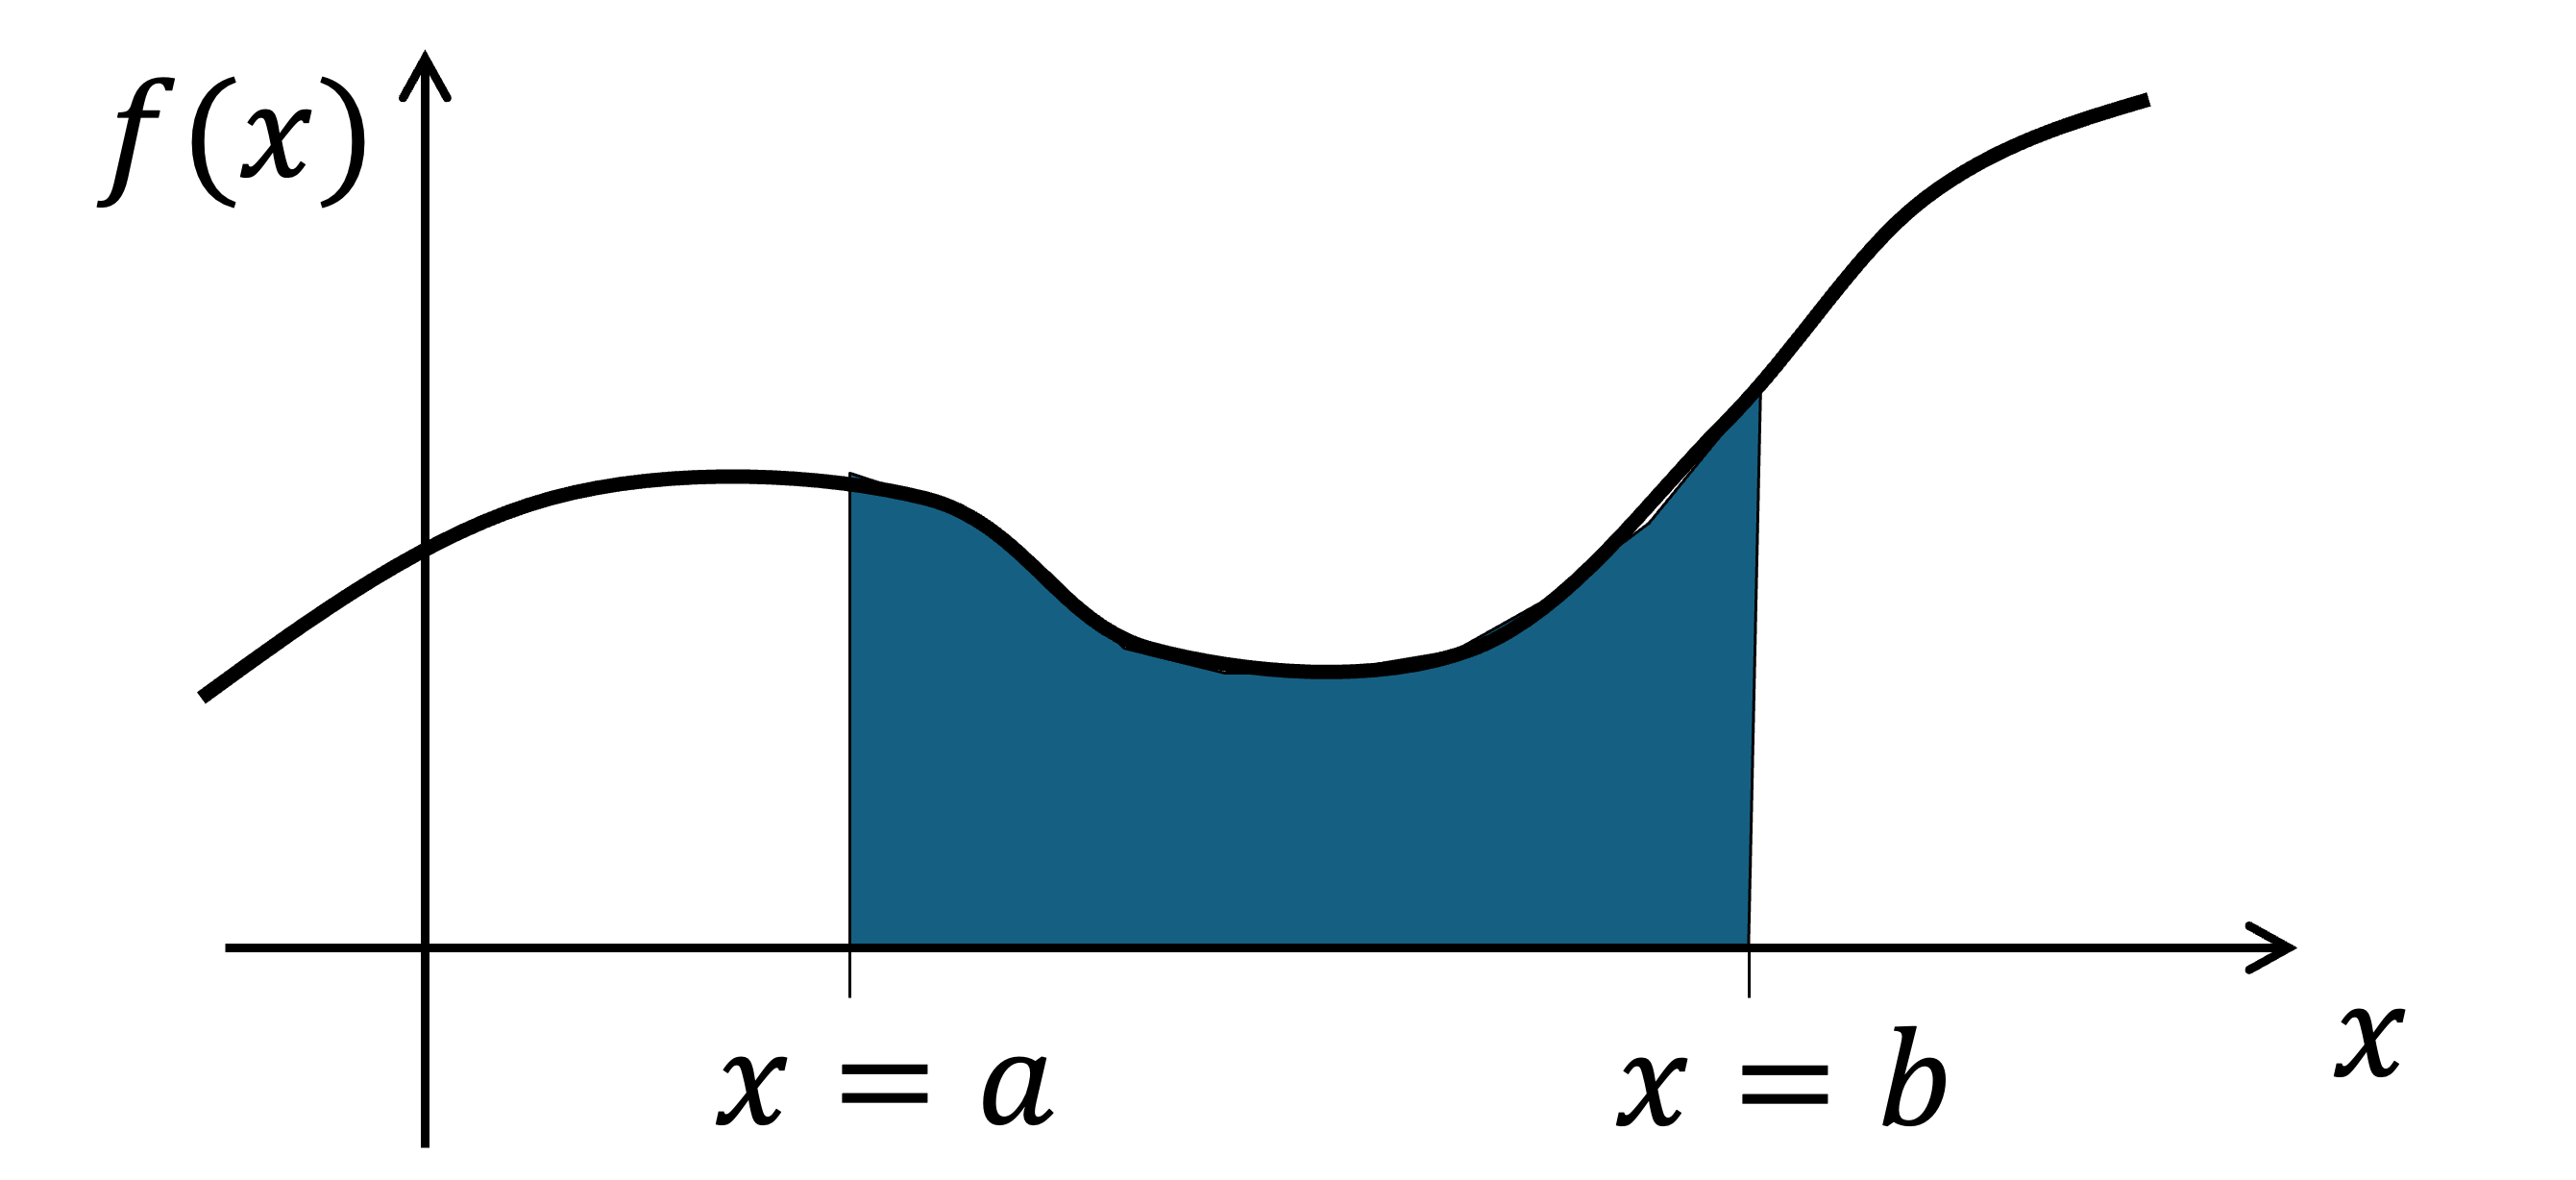
\includegraphics[width=0.5\textwidth]{Figures/Section3/312_areaunder.png}
    \caption{Sketch showing the area under the curve $f(x)$ given by $\int_a^b f(x) \, {\rm d} x$.}
    \label{fig:int_curve}
\end{figure}

The area under the curve (\textit{i.e.} between the curve and the $x$-axis) for $a\leq x\leq b$ is given by the integral
\[
A=\int_a^b f(x)\,{\rm d}x.
\]

\begin{example}[DIY]
Find the area under the curve
\[
f(x)=6x^2
\]
between $2\leq x\leq5$.
\end{example}

\begin{blanksol}
The indefinite integral is
\[
F(x)=\int f(x)\,{\rm d}x=\int 6x^2\,{\rm d}x
\]
\[
=2x^3+C.
\]
Evaluating at the limits and subtracting
\[
F(5)-F(2)=2\left(5^3-2^3\right)=2\times117
\]
\[
=234.
\]
\end{blanksol}

\textbf{Area between curves.} The area under a curve is a special case of finding the area between two curves. The area is given by
\[
\int_a^b\left(f_2-f_1\right)\,{\rm d}x
\]
where $f_1$ is the lower curve and $f_2$ is the upper curve and $a$ and $b$ are the limits on the area (see figure \ref{fig:int_between}(a)).

When using this formula, be aware of points where the curves cross. The area will be subtracted for regions where $f_2(x)<f_1(x)$ (see figure \ref{fig:int_between}(a)).

\begin{figure}
    \centering
    \subfig{0.48}{Figures/Section3/32_area_between.png}{$f_2(x) > f_1(x)$ for $a \leq x \leq b$}
    \hfill
    \subfig{0.48}{Figures/Section3/32_area_between_cross.png}{$f_2(x)$ and $f_1(x)$ cross in the domain $a \leq x \leq b$}
    \caption{Visualisation of the area between curves $f_1(x)$ and $f_2(x)$ given by $\int_a^b [f_2(x)-f_1(x)] \, {\rm d} x$. Blue indicates a positive contribution to the integral, red a negative contribution. \textit{I.e.} in (b) the result is the blue area minus the red area.}
    \label{fig:int_between}
\end{figure}


\begin{example}[Lecture]
Find the area between the curves represented by
\[
f(x)=5x^2-13x+13
\]
and
\[
g(x)=2x+3.
\]
\begin{center}
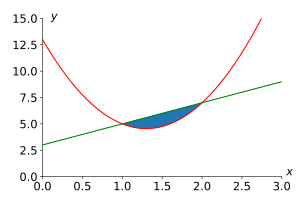
\includegraphics[width=0.5\textwidth, alt={Plot of f(x) and g(x) with shaded area showing the area between the curves.}]{Figures/Section3/Ex_322.png}
\end{center}
\end{example}

\begin{solution}
Find where $f(x)$ and $g(x)$ cross by solving $f(x)=g(x)$.
\begin{align*}
5x^2-13x+13 &=2x+3\\
\therefore\blank{5x^2-15x+10}&=0\\
\therefore\blank{5(x-1)(x-2)}&=0.
\end{align*}
Solving the quadratic gives $x=\blank{1}$ and $x=\blank{2}$.

Note that $g(x)$ passes above $f(x)$ and so the area between the curves is therefore
\begin{align*}
\int_{\blank{1}}^{\blank{2}}\left[g(x)-f(x)\right]{\rm d}x
&=\blank{\int_1^2\left(-5x^2+15x-10\right){\rm d}x} \\
&=\blank{\left[-\frac{5}{3}x^3 + \frac{15}{2}x^2-10x\right]_1^2}\\
&= \blank{\left[\frac{1}{6}(-80 + 180 - 120) - (-10 + 45 - 60)\right]}\\
&=\blank{\frac{5}{6}}.
\end{align*}
\end{solution}

\begin{recap}{\ref{sec:areas_int}}
\item The area \textbf{under the curve} for $a\leq x\leq b$ is
\[
A=\int_a^b f(x)\,{\rm d}x.
\]
\item The area \textbf{between two curves} is
\[
\int_a^b\left(f_2-f_1\right)\,{\rm d}x.
\]
\item This assumes $f_2>f_1$, so separate integrals are needed to deal with \textbf{crossing points}.
\end{recap}

\subsection{Improper integrals}
\label{sec:improper_int}

\begin{learningoutcomes}
\item Identify improper integrals
\item Use limits to investigate improper integrals
\end{learningoutcomes}

Consider the integral,
\[
\int_0^1 x^2\,{\rm d}x.
\]
\begin{itemize}
\item The integrand is finite
\item The limits are finite
\item The integrand can be integrated
\end{itemize}
This integral can be carried out without problems and so this is said to be a \textbf{proper integral}.

\textbf{Integrals with infinite limits.} An integral with an infinite limit, such as
\[
\int_a^\infty f(x)\,{\rm d}x
\qquad\text{or}\qquad
\int_{-\infty}^b f(x)\,{\rm d}x
\qquad\text{or}\qquad
\int_{-\infty}^\infty f(x)\,{\rm d}x,
\]
is said to be an \textbf{improper integral}. It \textbf{may} be possible to evaluate this integral or it may be infinite. 

Sometimes a geometrical consideration can be insightful. Consider the integral
\[
\int_1^\infty 1\, {\rm d}x.
\]
From the area under the curve (figure \ref{fig:improper_examples}(a)), it can be seen that the integral is infinite, \textit{i.e.} this integral cannot be evaluated, its value is not defined. Instead, consider the integral
\[
\int_1^\infty\frac{1}{x^2}\,{\rm d}x.
\]
The area under the curve is infinitely long but infinitely thin (figure \ref{fig:improper_examples}(b)). It is not clear whether the integral will be finite or infinite. 

\begin{figure}[h]
    \centering
    \subfig{0.33}{Figures/Section3/33_1int.png}{$\int_1^\infty 1\, {\rm d}x$}
    \hfill
    \subfig{0.63}{Figures/Section3/33_invxsq.png}{$\int_1^\infty\frac{1}{x^2}\,{\rm d}x$}
    \caption{Plots of the area under the curve for two example improper integrals.}
    \label{fig:improper_examples}
\end{figure}

Replacing the infinite limit with a parameter can usually be used to evaluate the integral. So, rather than $\int_1^\infty\frac{1}{x^2}\,{\rm d}x$, consider the integral $\int_1^u\frac{1}{x^2}\,{\rm d}x$ and take the limit as $u$ becomes very large:
\[
\int_1^\infty\frac{1}{x^2}\,{\rm d}x = \lim_{u\to\infty}\int_1^u\frac{1}{x^2}\,{\rm d}x.
\]
First, evaluate the substituted integral
\[
\int_1^u\frac{1}{x^2}\,{\rm d}x
=\left[-\frac{1}{x}\right]_1^u
=-\frac{1}{u}-\left(-\frac{1}{1}\right)
=1-\frac{1}{u}.
\]
Then, take the limit
\[
\lim_{u\to\infty}\int_1^u\frac{1}{x^2}\,{\rm d}x
=\lim_{u\to\infty}\left(1-\frac{1}{u}\right)
=1.
\]
Therefore, in this case we see that the integral \textbf{converges} to a value of $\int_1^\infty\frac{1}{x^2}\,{\rm d}x=1$.

On the other hand, consider $\int_1^\infty\frac{1}{x}\,{\rm d}x$. Making the substitution
\[
\int_1^u\frac{1}{x}\,{\rm d}x
=\left[\ln x\right]_1^u
=\ln u \, ,
\]
and so 
\[
\int_1^\infty\frac{1}{x}\,{\rm d}x = \lim_{u\to\infty}\ln u
\]
which becomes infinite, so this integral \textbf{does not converge}.

\begin{example}[Lecture]
Find out whether the following improper integrals converge
\begin{enumerate}
\item[(a)] $\displaystyle\int_1^\infty\frac{1}{x^3}\,{\rm d}x$
\item[(b)] $\displaystyle\int_1^\infty\frac{x}{1+x^2}\,{\rm d}x$
\end{enumerate}
and if so, to what value.

Hint:
\[
\int\frac{x}{1+x^2}\,{\rm d}x=\frac{1}{2}\ln(1+x^2)+C.
\]
\end{example}

\begin{solution}
(a) Substitute the upper limit of the integral and take the limit:
\[
\int_1^\infty\frac{1}{x^3}\,{\rm d}x
=\lim_{u\to\infty}\int_1^u x^{-3}\,{\rm d}x
=\lim_{u\to\infty}\blank{\left[-\frac{1}{2x^2}\right]_1^u}
\]
\[
=\lim_{u\to\infty}\blank{\left(\frac{1}{2}-\frac{1}{2u^2}\right)}
=\blank{\frac{1}{2}}.
\]

(b) Substitute the upper limit of the integral and calculate the integral:
\[
\int_1^\infty\frac{x}{1+x^2}\,{\rm d}x
=\lim_{u\to\infty}\int_1^u\frac{x}{1+x^2}\,{\rm d}x
=\lim_{u\to\infty}\blank{\left[\frac{1}{2}\ln(1+x^2)\right]_1^u}
\]
\[
=\lim_{u\to\infty}\blank{\frac{1}{2}\ln(1+u^2)-\frac{1}{2}\ln2}
=\blank{\infty}.
\]
\end{solution}

Sometimes, even when an integral cannot be calculated, it is possible to put some bounds on it by using an integral we can calculate.

\begin{example}[DIY]
Find lower and upper bounds on the integral
\[
\int_1^\infty\frac{\sin x}{x^2}\,{\rm d}x.
\]
\begin{center}
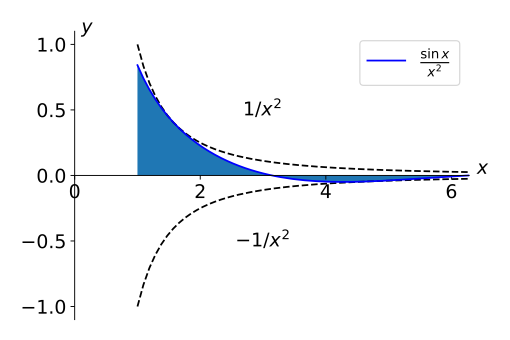
\includegraphics[width=0.6\textwidth,alt={Plot of $\sin x/x^2$}]{Figures/Section3/Ex332.png}
\end{center}
\end{example}

\begin{blanksol}
Since
\[
-1\leq\sin x\leq1,
\]
then
\[
-\frac{1}{x^2}\leq\frac{\sin x}{x^2}\leq\frac{1}{x^2}.
\]
We already showed $\int_1^{\infty} 1/x^2=1$, therefore
\[
-1\leq\int_1^\infty\frac{\sin x}{x^2}\,{\rm d}x\leq1.
\]
\end{blanksol}

\textbf{Improper Integrals with a singularity in the integrand.} Consider now the integral
\[
\int_{-1}^1\frac{1}{x(1-x^2)}\,{\rm d}x \,.
\]
Although the limits are finite, the integrand becomes infinite
\begin{itemize}
\item at either limit
\item at a point between the limits
\end{itemize}
as shown in figure \ref{fig:improper_sing}. When either of these are true, it is an \textbf{improper integral}.

\begin{figure}[h]
    \centering
    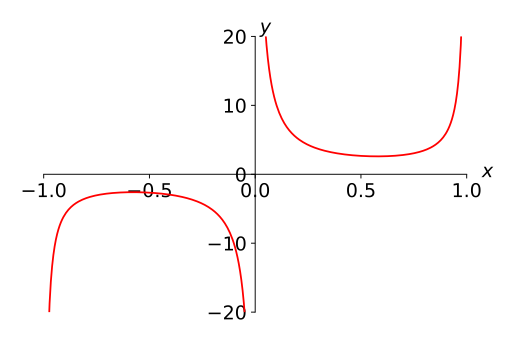
\includegraphics[width=0.5\textwidth]{Figures/Section3/33_implicit_sing.png}
    \caption{Plot of the function $\frac{1}{x(1-x^2)}$ which goes to infinity at $x = -1$, $0$, and $1$.}
    \label{fig:improper_sing}
\end{figure}

To evaluate such an integral, once again the concept of a limit can be used. Consider the simpler integral $\int_0^1\frac{1}{x}\,{\rm d}x$ where the integrand is infinite at $x=0$. Rewrite as
\[
\int_0^1\frac{1}{x}\,{\rm d}x
=\lim_{u\to0}\int_u^1\frac{1}{x}\,{\rm d}x
=\lim_{u\to0}\left[\ln x\right]_u^1
=\lim_{u\to0}(-\ln u),
\]
which does not converge as $\ln(0)$ does not exist.

\begin{example}[Video]
Investigate the improper integrals
\[
\int_0^1\frac{1}{x^3}\,{\rm d}x
\]
and
\[
\int_0^1\frac{1}{\sqrt{x}}\,{\rm d}x
\]
to determine whether they converge, and if so, to what value.

\begin{center}
   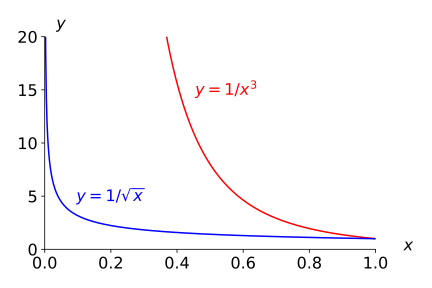
\includegraphics[width=0.5\textwidth, alt={Plot of the two integrands in this example.}]{Figures/Section3/Ex333.png} 
\end{center}
\end{example}

\begin{solution}
Both integrands diverge as $x\to0$, so we evaluate in the limit. First case:
\[
\int_0^1\frac{1}{x^3}\,{\rm d}x
=\lim_{u\to0}\int_u^1x^{-3}\,{\rm d}x
=\lim_{u\to0}\blank{\left[-\frac{x^{-2}}{2}\right]_u^1}
\]
\[
=\lim_{u\to0}\left(\blank{\frac{1}{2u^2}-\frac{1}{2}}\right)
=\blank{\text{undefined}}.
\]
In the second case
\[
\int_0^1\frac{1}{\sqrt{x}}\,{\rm d}x
=\lim_{u\to0}\int_u^1x^{-1/2}\,{\rm d}x
=\lim_{u\to0}\blank{\left[2x^{1/2}\right]_u^1}
\]
\[
=\lim_{u\to0}\left(\blank{2-2u^{1/2}}\right)=\blank{2}.
\]
\end{solution}

\textbf{Convergence of $x^n$.} For which values of $n$ do the following integrals converge?
\begin{enumerate}
\item[(a)] $\displaystyle\int_0^1x^n\,{\rm d}x$
\item[(b)] $\displaystyle\int_1^\infty x^n\,{\rm d}x$
\item[(c)] $\displaystyle\int_0^\infty x^n\,{\rm d}x$.
\end{enumerate}

First, let's calculate the indefinite integral, remembering the special case when $n=-1$
\[
\int x^n\,{\rm d}x=
\begin{cases}
\dfrac{x^{n+1}}{n+1}+C,& n\neq-1,\\[2mm]
\ln|x|+C,& n=-1.
\end{cases}
\]

(a) The integrand has a singularity at $x=0$ if $n<0$. From the indefinite integral
\[
\int_0^1x^n\,{\rm d}x = 
\begin{cases}
\dfrac{1}{n+1} - \lim_{x\to0}\dfrac{x^{n+1}}{n+1},& n\neq-1,\\[2mm]
-\lim_{x\to0}\ln|x|,& n=-1.
\end{cases}
\]
Inspecting the limits $\lim_{x\to0}\frac{x^{n+1}}{n+1}$, converges if $n>-1$ and does not converge otherwise. Additionally, $\lim_{x\to0}\ln|x|$ does not converge. So, $\int_0^1x^n\,{\rm d}x$ \textbf{converges for $n>-1$}. See figure \ref{fig:xpown_improper}(a) for some example curves.

(b) The integrand goes to infinity as $x\to\infty$ if $n>0$. From the indefinite integral
\begin{align*}
\int_1^\infty x^n\,{\rm d}x = 
\begin{cases}
\lim_{x\to\infty}\dfrac{x^{n+1}}{n+1} - \dfrac{1}{n+1},& n\neq-1,\\[2mm]
\lim_{x\to\infty}\ln|x|,& n=-1.
\end{cases}
\end{align*}
Inspecting the limits $\lim_{x\to\infty}\frac{x^{n+1}}{n+1}$, converges if $n<-1$ and does converge not otherwise. Additionally, $\lim_{x\to\infty}\ln|x|$ does not converge. So, $\int_1^\infty x^n\,{\rm d}x$ \textbf{converges for $n<-1$}. See figure \ref{fig:xpown_improper}(b) for some example curves.

(c) The integrand goes to infinity as $x\to0$ if $n<0$ and as $x\to\infty$ if $n>0$. We can split the limits to write the integral as the sum of the integrals in (a) and (b)
\[
\int_0^\infty x^n\,{\rm d}x
=\int_0^1x^n\,{\rm d}x+\int_1^\infty x^n\,{\rm d}x.
\]
The first integral only converges for $n>-1$. The second integral only converges for $n<-1$, therefore
\[
\int_0^\infty x^n\,{\rm d}x
\]
\textbf{does not converge for any} $n$.

\begin{figure}[h]
\centering
    \subfig{0.48}{Figures/Section3/33_xn.png}{$\int_0^1 x^n\,{\rm d}x$}
    \hfill
    \subfig{0.48}{Figures/Section3/33_xn2.png}{$\int_1^\infty x^n\,{\rm d}x$}
    \caption{Plots of various functions of the form $x^n$ between the limits (a) $0 \leq x \leq 1$ and (b) $x \geq 1$. The green curves show those which result in a convergent improper integral in the limits labelled, while the integrals of the red curves do not converge.}
    \label{fig:xpown_improper}
\end{figure}

\textbf{Singularity between the limits of integration.} If there is a place between the limits where the integrand is infinite, then the integral should be split at that point and the parts evaluated separately. If any of the parts does not converge then the whole integral does not converge.


\begin{exammistake} 
Assuming that the integral cannot be evaluated if the integrand is infinite. 
\begin{quote}
    \textbf{25/26 Exam Q3(a)(ii)} \[ f(x)=3x+1+\frac{2}{x-3}-\frac{4}{x+2}. \] Determine whether \[ \int_4^6 f(x)\,dx \] and \[ \int_0^3 f(x)\,dx \] converge to a value and, if so, find the value.
\end{quote}
The second integral does not converge, but the reason is not ``because \(\dfrac{2}{x-3}\) is undefined at \(x=3\)'' it is because \(2\ln|x-3|\) is undefined at \(x=3\). 

In this case this still resulted in the correct response, but would be incorrect if the term was \textit{e.g.} $\frac{2}{\sqrt{x-3}}$.
\end{exammistake}

\begin{example}[Lecture]
Consider the improper integral
\[
\int_{-1}^1\frac{1}{x^2}\,{\rm d}x.
\]
\begin{enumerate}
\item[(a)] Determine whether it converges. If so, find its value.
\item[(b)] Compare this to the result you would find if you did not split the integral.
\end{enumerate}
\end{example}

\begin{solution}
(a) Calculate the indefinite integral
\[
\int x^{-2}\,{\rm d}x=\blank{-\frac{1}{x}+C}.
\]
Split the integral at the point where the integrand diverges:
\[
\int_{-1}^1\frac{1}{x^2}\,{\rm d}x
=\int_{-1}^0\frac{1}{x^2}\,{\rm d}x+\int_0^1\frac{1}{x^2}\,{\rm d}x.
\]
Evaluate the integrals in the limit where the upper/lower limit of integration goes to 0:
\[
\lim_{u\to0^-}\left[\blank{-\frac{1}{x}}\right]_{-1}^{u}
=\blank{\infty},
\]
\[
\lim_{u\to0^+}\left[\blank{-\frac{1}{x}}\right]_{u}^{1}
=\blank{\infty}.
\]
Therefore, $\int_{-1}^1\frac{1}{x^2}\,{\rm d}x$ does not converge.

(b) Na{\"i}vely substituting in the limits of integration gives
\[
\left[\blank{-\frac{1}{x}}\right]_{-1}^{1}=\blank{-2},
\]
which is misleading (and wrong!) because the integral must be split at the singularity.
\end{solution}

\begin{recap}{\ref{sec:improper_int}}
\item A definite integral is improper if
\begin{itemize}
\item Either or both \textbf{limits are infinite}
\item The \textbf{integrand becomes infinite} between or at the limits
\end{itemize}
\item Improper integrals \textbf{may converge to a solution}, or may not.
\item To investigate an improper integral, \textbf{substitute} the problem limit(s) for a variable \textbf{then take the limit} of that variable going to the original.
\end{recap}

\subsection{Further rules of integration}
\label{sec:further_int}

\begin{learningoutcomes}
\item Use integration by substitution to evaluate appropriate integrals
\item Recall and apply the formula for integration by parts
\item Use partial fractions to evaluate integrals involving rational fractions
\end{learningoutcomes}

\subsubsection{Integration by substitution} 

In some cases, substituting the variable in an integral appropriately can make it easier to evaluate. In a sense, integration by substitution is like differentiating using the chain rule, but in reverse.

For example, consider the derivative of $\sin(x^2)$:
\[
\der{}{x}\sin(x^2)=\cos(x^2)\times\der{}{x}x^2=2x\cos(x^2).
\]
So,
\[
\int 2x\cos(x^2)\,{\rm d}x=\sin(x^2)+C.
\]
But how to find this result without being given the answer to start with?

Start with the integral
\[
\int 2x\cos(x^2)\,{\rm d}x.
\]
We can see that the cosine is acting on $x^2$, so this is the candidate for our ``inner function''. So, substitute $x^2$ for a new variable, call it $u$, and rearrange the integral in terms of $u$.
\[
u=x^2 \quad\text{and so}\quad \der{u}{x}=2x
\qquad \therefore \; {\rm d}u=2x\,{\rm d}x.
\]
Therefore, the integral becomes
\begin{align*}
\int\cos u\,{\rm d}u &=\sin u+C\\
&=\sin(x^2)+C.
\end{align*}

More generally, for an integral of the form
\[
\int f(g(x))g'(x)\,{\rm d}x,
\]
a substitution $u=g(x)$ can be used, resulting in the integral $\int f(u)\,{\rm d} u$. If this integral can be evaluated for $u$, then $u=g(x)$ can be substituted back into the result to give the solution in terms of $x$.

This can also be derived directly from the chain rule. Starting with a function of the form $y=F(g(x))$, the chain rule gives $\der{y}{x} = g'(x)F'(g(x))$. Therefore,
\[
\int f[g(x)]g'(x)\,{\rm d}x=F(g(x))+C,
\]
where $f(u)=F'(u)$.

\begin{example}[DIY]
Using a substitution, evaluate the integral
\[
\int\frac{(\ln x)^5}{x}\,{\rm d}x.
\]
\end{example}

\begin{blanksol}
Define $u=\ln(x)$, and so ${\rm d}u=\dfrac{1}{x}\,{\rm d}x$. Substituting this in gives
\[
\int\frac{(\ln x)^5}{x}\,{\rm d}x=\int u^5\,{\rm d}u=\frac{u^6}{6}+C.
\]
Substituting $u=\ln(x)$ back in gives
\[
\int\frac{(\ln x)^5}{x}\,{\rm d}x=\frac{1}{6}(\ln x)^6+C.
\]
\end{blanksol}

\textbf{Definite Integration by substitution.} To evaluate a definite integral by substitution, the limits must be expressed in terms of the new variable. For example,
\[
\int_0^2x^2(x^3+5)^4\,{\rm d}x,
\]
use the substitution $u(x)=x^3+5$ so that ${\rm d}u=3x^2\,{\rm d}x$ and the integral becomes $\int\frac{1}{3}u^4\,{\rm d}u$. The limits need to be converted to $u$ values. $u(0)=5$ and $u(2)=13$, so the integral becomes
\[
\int_5^{13}\frac{1}{3}u^4\,{\rm d}u
=\frac{1}{15}\left[u^5\right]_5^{13}
=\frac{13^5-5^5}{15}
=\frac{368168}{15}.
\]

\begin{example}[Lecture]
Using substitution, evaluate the integral
\[
\int_0^{1/2}x\cos(\pi x^2)\,{\rm d}x.
\]
\end{example}

\begin{solution}
Substitute $u=\blank{\pi x^2}$, then $u'=\blank{2\pi x}$.

The limits of the integral become $u(0)=\blank{0}$ and $u(1/2)=\blank{\pi/4}$.

As ${\rm d}u=u'\,{\rm d}x$, then ${\rm d}x=\dfrac{1}{2\pi x}\,{\rm d}u$, substituting gives
\begin{align*}
    \int_0^{1/2}x\cos(\pi x^2)\,{\rm d}x
    &=\blank{\int_0^{\pi/4}\frac{x}{2\pi x}\cos u\,{\rm d}u} \\
    &=\blank{\frac{1}{2\pi}\int_0^{\pi/4}\cos u\,{\rm d}u}\, .
\end{align*}

Evaluating the integral in $u$ we get
\[
\blank{\frac{1}{2\pi}\int_0^{\pi/4}\cos u\,{\rm d}u
=\frac{1}{2\pi}\left[\sin u\right]_0^{\pi/4}
=\frac{1}{2\pi}\times\frac{\sqrt{2}}{2}}
\]
\[
=\blank{\frac{\sqrt{2}}{4\pi}.}
\]
\end{solution}

\begin{example}[Video]
A cylindrical tube of diameter 8cm and length 1m, held horizontally, is partially filled with water to a depth of 2cm.

Use integration to calculate the volume of water in the tube.
\begin{center}
    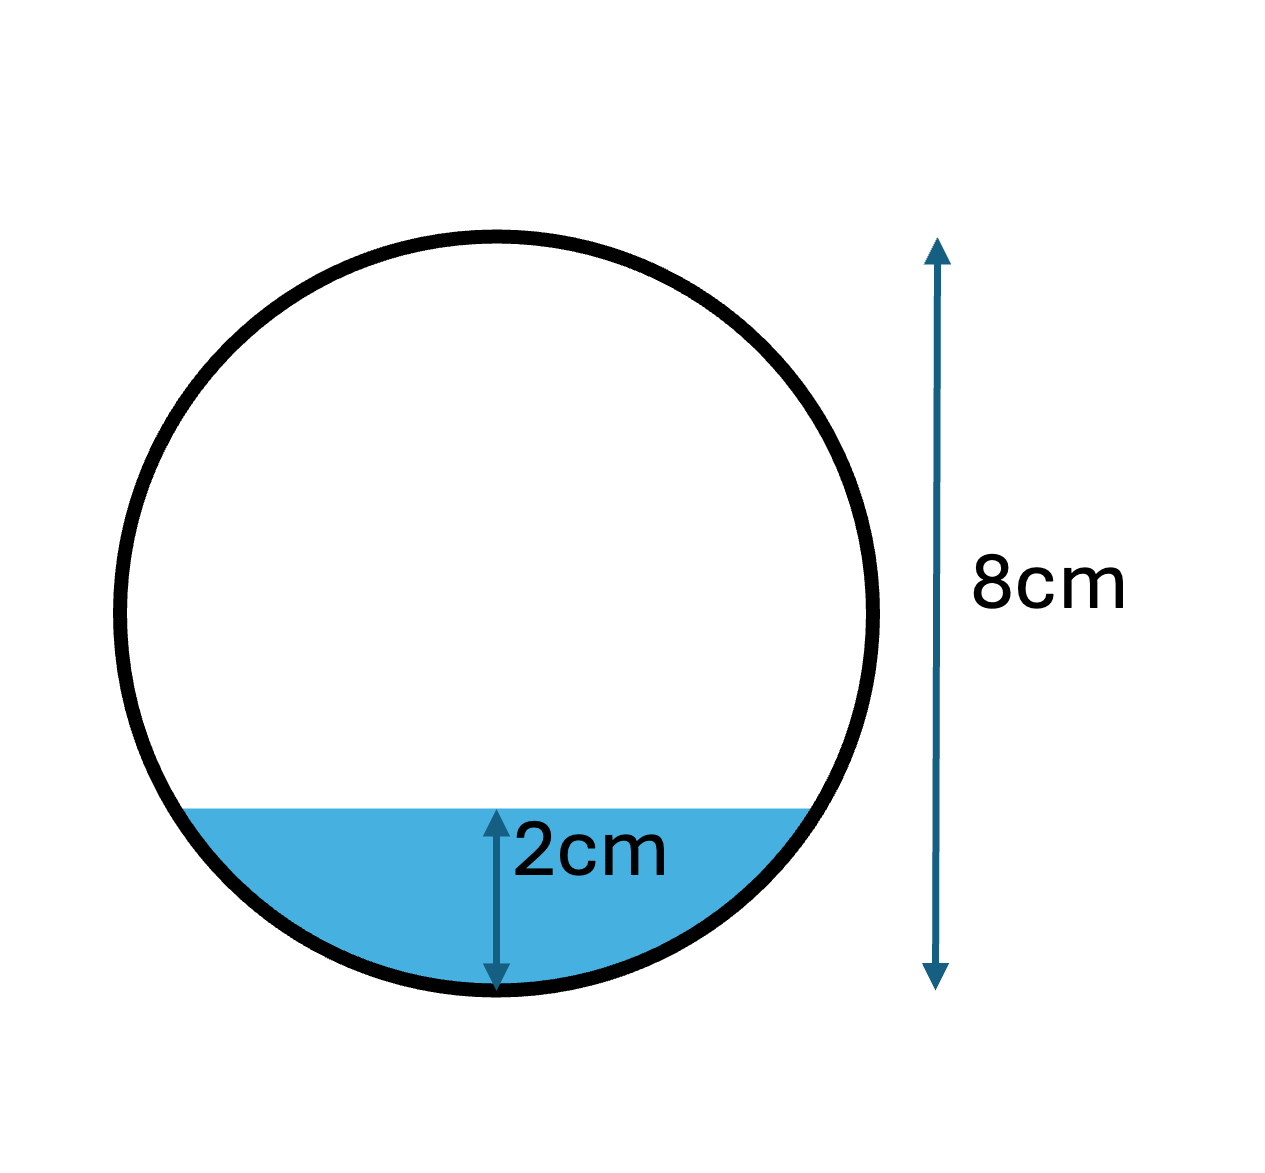
\includegraphics[width=0.3\textwidth,alt={Sketch of the tube cross section.}]{Figures/Section3/Ex343.png}
\end{center}
\end{example}

\begin{solution}
The cross section of the tube is a circle with radius $R=4$cm, so can be represented by the equation:
\[
\blank{x^2+y^2=16}
\]
where the circle centre is at the origin $(0,0)$.

The surface of the water lies on the straight horizontal line
\[
\blank{y=-2}.
\]

We need to compute the integral below this curve and above the lower half of the circle, which is given by
\[
y=\blank{-\sqrt{16-x^2}}.
\]

To find the limits of integration, find where the two curves cross by substituting the equation for the line into the circle
\[
\blank{x^2+(-2)^2=16}
\qquad \therefore \;
\blank{x^2=12}.
\]
\[
x=\pm\blank{2\sqrt{3}}.
\]

Integrating the horizontal line gives the (negative) of the area above it
\[
A_1=\blank{\int_{-2\sqrt{3}}^{2\sqrt{3}}-2\,{\rm d}x}
=\blank{-8\sqrt{3}}.
\]

Next, we need to integrate the lower semi-circle
\[
A_2=\blank{-\int_{-2\sqrt{3}}^{2\sqrt{3}}\sqrt{16-x^2}\,{\rm d}x}.
\]

Using the substitution $x=\blank{4\sin\left(\frac{t}{2}\right)}$ then ${\rm d}x=\blank{2\cos\left(\frac{t}{2}\right)}\,{\rm d}t$.

The limits of the integral are at
\[
t=\blank{2\sin^{-1}\left(\pm\frac{\sqrt{3}}{2}\right)=\pm\frac{2\pi}{3}}.
\]

\[
A_2=\blank{-\int_{-2\pi/3}^{2\pi/3}4\sqrt{1-\sin^2\left(\frac{t}{2}\right)}
\times2\cos\left(\frac{t}{2}\right)\,dt
=-8\int_{-2\pi/3}^{2\pi/3}\cos^2\left(\frac{t}{2}\right)\,dt}.
\]

Using the trigonometric identity
\[
\blank{\cos^2\theta=\frac{1+\cos2\theta}{2}}
\]
this becomes
\[
A_2=\blank{-4\int_{-2\pi/3}^{2\pi/3}(1+\cos t)\,dt
=-4\left[t+\sin t\right]_{-2\pi/3}^{2\pi/3}
=-\frac{16\pi}{3}-8\sin\left(\frac{2\pi}{3}\right)}.
\]

Therefore, the area of the cross section filled by water is
\[
A_1-A_2=\blank{-8\sqrt{3}+\frac{16\pi}{3}+8\sin\left(\frac{2\pi}{3}\right)
\approx9.83\;\mathrm{cm}^2}.
\]

So the volume of water is approximately
\[
\blank{100\times9.83=983\;\mathrm{cm}^3\text{ or }983\mathrm{ml}}.
\]
\end{solution}

\subsubsection{Integration by parts} 

Often, a product of two functions can be integrated using a process known as `integration by parts'. In a sense, integrating by parts is the reverse of differentiating using the product rule.

The basic formula for integration by parts can be derived from the product rule. Start with the function
\[
y=u(x)v(x) \qquad\text{therefore}\qquad y'(x)=u'(x)v(x)+u(x)v'(x).
\]
Taking the integral of both sides gives $\int y'(x)\,{\rm d}x=\int u'(x)v(x)\,{\rm d}x+\int u(x)v'(x)\,{\rm d}x.$ Noting that $\int y'(x)\,{\rm d}x=y=u(x)v(x)$, we arrive at the formula for integration by parts
\begin{equation}
\label{eq:ibp} \int u(x)v'(x)\,{\rm d}x=u(x)v(x)-\int u'(x)v(x)\,{\rm d}x.
\end{equation}
It can be used to integrate a product by defining one factor as $u(x)$ and the other as $v'(x)$, with the aim of making the resulting integral easier.

Take the integral $\int x\sin x\,{\rm d}x$, let $u(x)=x$ and $v'(x)=\sin x$. Thus, $u'(x)=1$ and $v(x)=-\cos x$. Using equation \eqref{eq:ibp}
\begin{align*}
\int x\sin x\,{\rm d}x &= -x\cos x+\int\cos x\,{\rm d}x.\\
&=-x\cos x+\sin x+C.
\end{align*}

Sometimes, integration by parts needs to be used more than once. For example, the function $x^2\cos x$ integrates (using equation \eqref{eq:ibp} with $u=x^2$ and $v=\cos x$) to
\begin{align*}
    \int x^2\cos x\,{\rm d}x &= x^2\sin x-\int2x\sin x\,{\rm d}x\\
    &= x^2\sin x-\left(-2x\cos x+\int2\cos x\,{\rm d}x\right)\\
    &=(x^2-2)\sin x+2x\cos x+C.
\end{align*}

\begin{example}[Lecture]
Using integration by parts, find
\[
\int e^x\sin x\,{\rm d}x.
\]
\end{example}

\begin{solution}
Define $u=\sin x$ and $v'=e^x$. Then $u'=\blank{\cos(x)}$ and $v=\blank{e^x}$.

Using equation \eqref{eq:ibp} $\int uv'\,{\rm d}x=uv-\int u'v\,{\rm d}x$ so,
\[
\int e^x\sin x\,{\rm d}x=\blank{e^x\sin x}-\int \blank{e^x\cos x}\,{\rm d}x. \tag{1}
\]
Now define $u=\cos(x)$ and $v'=e^x$. Then $u'=\blank{-\sin(x)}$ and $v=\blank{e^x}$.
\[
\int e^x\cos x\,{\rm d}x=\blank{e^x\cos x} + \int \blank{e^x\sin x}\,{\rm d}x. \tag{2}
\]
Define $I=\int e^x\sin x\,{\rm d}x$ then we can write equation (2) as
\[
\int e^x\cos x\,{\rm d}x = \blank{e^x\cos x+I}.
\]
Substituting into equation (1),
\[
I=\blank{e^x\sin x-e^x\cos x-I}
\qquad \therefore \;
\blank{2I=e^x(\sin x-\cos x)}\, .
\]
And so
\[
\int e^x\sin x\,{\rm d}x=\blank{\frac{e^x}{2}(\sin x-\cos x)+C}.
\]
\end{solution}

Usually, if the integrand is a product with a polynomial, then the polynomial is taken to be $u(x)$ so that $u'(x)$ will present a simpler integral. An exception is if the other factor is a logarithm or an inverse trigonometric function.

For example, to find $\int x^2\ln x\,{\rm d}x$, define $u(x)=\ln x$ and $v'(x)=x^2$, so that $u'(x)=\frac{1}{x}$ and $v(x)=\frac{x^3}{3}$. Using equation \eqref{eq:ibp} the integral becomes
\begin{align*}
    \int x^2\ln x\,{\rm d}x &= \frac{1}{3}x^3\ln x-\int\frac{x^3}{3x}\,{\rm d}x\\
    &=\frac{1}{3}x^3\ln x-\frac{1}{3}\int x^2\,{\rm d}x\\
    &= \frac{1}{3}x^3\ln x-\frac{1}{9}x^3+C.
\end{align*}

\begin{example}[Lecture]
Using integration by parts, find
\[
\int\tan^{-1}x\,{\rm d}x.
\]
\end{example}

\begin{solution}
Define $u=\tan^{-1}x$ and $v'=1$. Then $u'=\blank{\dfrac{1}{1+x^2}}$ and $v=\blank{x}$.

Using the formula for IBP (equation \eqref{eq:ibp})
\[
\int\tan^{-1}x\,{\rm d}x=\blank{x\tan^{-1}x}-\int\blank{\frac{x}{1+x^2}}\,{\rm d}x.
\]
Using the substitution $z=x^2$, and so $dz=\blank{2x\,{\rm d}x}$,
\begin{align*}
    \int\frac{x}{1+x^2}\,{\rm d}x&=\blank{\frac{1}{2}\int\frac{1}{1+z}\,{\rm d}z}\\
    &=\blank{\frac{1}{2}\ln(1+z) = \frac{1}{2}\ln(1+x^2)}.
\end{align*}
Therefore,
\[
\int\tan^{-1}x\,{\rm d}x=\blank{x\tan^{-1}x-\frac{1}{2}\ln(1+x^2)+C}.
\]
\end{solution}

\[
\int u(x)v'(x)\,{\rm d}x=u(x)v(x)-\int u'(x)v(x)\,{\rm d}x.
\]
Note that, to carry out definite integration using integration by parts, all terms need to be evaluated at the limits, so
\[
\int_a^b u(x)v'(x)\,{\rm d}x=\left[u(x)v(x)\right]_a^b-\int_a^b u'(x)v(x)\,{\rm d}x.
\]

\subsubsection{Integration by partial fractions} 
\label{sec:IBpartfrac}

If a function can be expressed in terms of partial fractions, then these partial fractions can generally be integrated.

\begin{example}[Video]
Find
\[
\int\frac{x+17}{(x+3)(2x-1)}\,{\rm d}x
\]
using integration by partial fractions.
\end{example}

\begin{solution}
First write the partial fractions form
\[
\frac{x+17}{(x+3)(2x-1)}=\blank{\frac{A}{x+3}+\frac{B}{2x-1}}\, .
\]
Multiply through by the denominator
\[
x+17=\blank{A(2x-1)+B(x+3)}\, .
\]
Setting $x=-3$ allows us to find $A$:
\[
\blank{14=-7A \qquad\therefore\qquad A=-2}.
\]
Setting $x=1/2$ allows us to find $B$:
\[
\blank{\frac{35}{2}=\frac{7}{2}B \qquad\therefore\qquad B=5}.
\]
Now evaluate the integral
\begin{align*}
    \int\frac{x+17}{(x+3)(2x-1)}\,{\rm d}x
    &=\blank{-2\int\frac{1}{x+3}\,{\rm d}x+5\int\frac{1}{2x-1}\,{\rm d}x}\\
    &= \blank{-2\ln|x+3|+\frac{5}{2}\ln|2x-1|+C}.
\end{align*}
\end{solution}

\begin{recap}{\ref{sec:further_int}}
\item \textbf{Integration by substitution} is useful for integrands that can be expressed in the form
\[
\int f(g(x))g'(x)\,{\rm d}x.
\]
\item \textbf{Integration by parts} is used for integrating products of functions
\[
\int u(x)v'(x)\,{\rm d}x=u(x)v(x)-\int u'(x)v(x)\,{\rm d}x.
\]
\item \textbf{Partial fractions} can be used to make suitable integrals easier.
\end{recap}

\subsection{Double integrals over rectangular regions}
\label{sec:double_int}

\begin{learningoutcomes}
\item Calculate the volume under a surface with rectangular bounds using integration
\end{learningoutcomes}

The integral $\int_a^b f(x)\,{\rm d}x$ represents the area under the curve $y=f(x)$ between $x=a$ and $x=b$. Consider instead a function of two variables $f(x,y)$. The integral
\[
\int_c^d f(x,y)\,{\rm d}x
\]
represents the area of a slice at position $y$. Multiplying by ${\rm d}y$ gives $\left(\int_c^d f(x,y) \,{\rm d}x\right) \,{\rm d}y$ representing the volume of a slice at position $y$ with infinitesimal thickness ${\rm d}y$. The sum of all slices between $y=a$ and $y=b$ is given by the integral of the integral, \emph{i.e.}
\begin{equation}
    \label{eq:doubleint} \int_a^b\int_c^d f(x,y)\,{\rm d}x\,{\rm d}y \, .
\end{equation}

The double integral in equation \eqref{eq:doubleint} represents the volume underneath the function but above the rectangle $z=0$; $a\leq y\leq b$; $c\leq x\leq d$.

Figure \ref{fig:double_integrals} illustrates the double integration process.

\textbf{Inner and outer integral.} From the definition in equation \eqref{eq:doubleint} the integral $\int_c^d f(x,y)\,{\rm d}x$
is known as the `inner integral'. It can be evaluated and will be a function of $y$
\[
\int_c^d f(x,y)\,{\rm d}x=g(y).
\]
To find $g(y)$, treat $y$ as a constant and integrate with respect to $x$. \emph{E.g.} If $f(x,y)=e^x\cos y$, then
\[
\int_c^d f(x,y)\,{\rm d}x=\cos y\left[e^d-e^c\right].
\]

Once the inner integral is evaluated it can be placed in the main integral to give
\[
\int_a^b g(y)\,{\rm d}y.
\]
This is known as the `outer integral'.

Note that reversing the order of the integrations (along with their limits) preserves the integral, \emph{i.e.}
\[
\int_a^b\int_{x=c}^d f(x,y)\,{\rm d}x\,{\rm d}y
=
\int_c^d\int_{y=a}^b f(x,y)\,{\rm d}y\,{\rm d}x.
\]

\begin{figure}[h]
    \centering
    \subfig{0.32}{Figures/Section3/35_doubleint1.png}{Area of  a strip}
    \hfill
    \subfig{0.32}{Figures/Section3/35_doubleint2.png}{Volume of a strip}
    \hfill
    \subfig{0.32}{Figures/Section3/35_doubleint3.png}{Volume under the surface}
    \\
    \subfig{0.32}{Figures/Section3/35_double_topdown1.png}{$\int_c^d f(x,y)\,{\rm d}x$}
    \hfill
    \subfig{0.32}{Figures/Section3/35_double_topdown2.png}{$\left(\int_c^d f(x,y)\,{\rm d}x\right)\,{\rm d}y$}
    \hfill
    \subfig{0.32}{Figures/Section3/35_double_topdown3.png}{$\int_a^b\int_{x=c}^d f(x,y)\,{\rm d}x\,{\rm d}y$}
    \caption{Building up the double integral to find the volume under a surface step-by-step from (a)--(c) three-dimensional view and (d)--(f) looking down from above.}
    \label{fig:double_integrals}
\end{figure}

\begin{example}[DIY]
Find the double integral
\[
\int_{-\pi}^{\pi}\int_0^1 (x^2+2x-1)\cos\left(\frac{y}{2}\right)\,{\rm d}x\,{\rm d}y
\]
and show it is the same if the order of integration is reversed
\[
\int_0^1\int_{-\pi}^{\pi}(x^2+2x-1)\cos\left(\frac{y}{2}\right)\,{\rm d}y\,{\rm d}x.
\]
\end{example}

\begin{blanksol}
Take the first case and evaluate the inner integral, treating $y$ as constant:
\[
\int_0^1(x^2+2x-1)\cos\left(\frac{y}{2}\right)\,{\rm d}x
=
\cos\left(\frac{y}{2}\right)
\left[\frac{x^3}{3}+x^2-x\right]_0^1
=
\frac{1}{3}\cos\left(\frac{y}{2}\right).
\]
Now evaluate the outer integral:
\[
\frac{1}{3}\int_{-\pi}^{\pi}\cos\left(\frac{y}{2}\right)\,{\rm d}y
=
\frac{2}{3}\left[\sin\left(\frac{y}{2}\right)\right]_{-\pi}^{\pi}
=
\frac{4}{3}.
\]

Reversing the order and evaluating the inner integral first:
\[
\int_{-\pi}^{\pi}(x^2+2x-1)\cos\left(\frac{y}{2}\right)\,{\rm d}y
=
(x^2+2x-1)
\left[2\sin\left(\frac{y}{2}\right)\right]_{-\pi}^{\pi}
\]
\[
=4(x^2+2x-1).
\]
Now evaluate the outer integral:
\[
4\int_0^1(x^2+2x-1)\,{\rm d}x
=
4\left[\frac{x^3}{3}+x^2-x\right]_0^1
=
\frac{4}{3}.
\]
\end{blanksol}

\begin{example}[Video]
An experiment is set up to measure the diffusion coefficient of benzene in water.

The flux at the outlet $F$ is measured, and should be given approximately by
\[
\frac{Fh}{D}=\int_0^l\int_0^l c(x,y)\,{\rm d}x\,{\rm d}y
\]
where $D$ is the diffusion constant and $c(x,y)$ the concentration at the inlet.

To correctly estimate $D$, the experiment is meant to keep $c(x,y)=c_0$ (a constant). However, due to an error in the setup, the actual concentration is
\[
c(x,y)=\left(\frac{3}{4}x^2+y+xy\right)c_0.
\]
Given that $F$ is measured to be $2.5$ [mol/s], $h=0.04$ [cm], $l=1$ [cm] and $c_0=10^4$ [mol/cm$^3$] find
\begin{itemize}
\item the real value of $D$ (using the actual concentration $c=\left(\frac{3}{4}x^2+y+xy\right)c_0$)
\item the value of $D$ obtained by the researchers (assuming $c=c_0$)
\end{itemize}
\end{example}

\begin{solution}
First take the case where
\[
c(x,y)=\left(\frac{3}{4}x^2+y+xy\right)c_0
\]
and compute the inner integral
\[
I(y)=\int_0^1c(x,y)\,{\rm d}x
=
\blank{c_0\left[\frac{1}{4}x^3+yx+\frac{1}{2}x^2y\right]_0^1}
\]
\[
=\blank{c_0\left(\frac{1}{4}+\frac{3}{2}y\right)}.
\]
Now compute the outer integral
\[
\frac{Fh}{D}=\int_0^1I(y)\,{\rm d}y
=
\blank{c_0\left[\frac{1}{4}y+\frac{3}{4}y^2\right]_0^1}
\]
\[
=\blank{c_0\times1=10^4\;[\mathrm{mol/cm}]}.
\]
Therefore,
\[
D=\blank{\frac{Fh}{c_0}=10^{-5}\;[\mathrm{cm}^2/\mathrm{s}]}.
\]

Now consider the intended setup where $c(x,y)=c_0$, the integration becomes
\[
\int_0^1\int_0^1c_0\,{\rm d}x\,{\rm d}y
=
\blank{c_0\int_0^1[x]_0^1\,{\rm d}y}
\]
\[
=\blank{c_0[y]_0^1=c_0=10^4\;[\mathrm{mol/cm}]}.
\]
and so
\[
D=\blank{\frac{Fh}{c_0}=10^{-5}\;[\mathrm{cm}^2/\mathrm{s}]}.
\]
So, we see that \blankpar{in both cases the result is the same, the researchers got lucky!}
\end{solution}

\begin{recap}{\ref{sec:double_int}}
\item The double integral
\[
\int_a^b\int_c^d f(x,y)\,{\rm d}x\,{\rm d}y
\]
consists of
\begin{itemize}
\item an \textbf{inner integral}: evaluated first to give
\[
\int_c^d f(x,y)\,{\rm d}x=g(y)
\]
\item and an \textbf{outer integral}: evaluated using the result
\[
\int_a^b g(y)\,{\rm d}y
\]
\end{itemize}
\item The result is the \textbf{volume} between the surface $z=f(x,y)$ and the plane $z=0$ in the \textbf{rectangular region} $a\leq y\leq b$; $c\leq x\leq d$.
\end{recap}

